\documentclass[11pt]{article}
\usepackage{geometry,marginnote} % Pour passer au format A4
\geometry{hmargin=1cm, vmargin=1.5cm} % 

% Page et encodage
\usepackage[T1]{fontenc} % Use 8-bit encoding that has 256 glyphs
\usepackage[english,french]{babel} % Français et anglais
\usepackage[utf8]{inputenc} 

\usepackage{lmodern}
\usepackage[np]{numprint}
\setlength\parindent{0pt}

% Graphiques
\usepackage{graphicx,float,grffile}
\usepackage{tikz,pst-eucl,pst-plot,pstricks,pst-node,pstricks-add,pst-fun,pgfplots} 

% Maths et divers
\usepackage{amsmath,amsfonts,amssymb,amsthm,verbatim,scratch3}
\usepackage{multicol,enumitem,url,eurosym,gensymb,tabularx}

\DeclareUnicodeCharacter{20AC}{\euro}



% Sections
\usepackage{sectsty} % Allows customizing section commands
\allsectionsfont{\centering \normalfont\scshape}

% Tête et pied de page
\usepackage{fancyhdr} \pagestyle{fancy} \fancyhead{} \fancyfoot{}

%\fancyfoot[L]{Collège Faubert}
%\fancyfoot[C]{\thepage / 6}
%\fancyfoot[R]{Série Générale}

\renewcommand{\headrulewidth}{0pt} % Remove header underlines
%\renewcommand{\footrulewidth}{0pt} % Remove footer underlines

\newcommand{\horrule}[1]{\rule{\linewidth}{#1}} % Create horizontal rule command with 1 argument of height

\newcommand{\Pointilles}[1][3]{%
  \multido{}{#1}{\makebox[\linewidth]{\dotfill}\\[\parskip]
}}

\newtheorem{Definition}{Définition}

\usepackage{siunitx}
\sisetup{
    detect-all,
    output-decimal-marker={,},
    group-minimum-digits = 3,
    group-separator={~},
    number-unit-separator={~},
    inter-unit-product={~}
}

\setlength{\columnseprule}{1pt}



\begin{document}



\begin{titlepage}

    \center % Center everything on the page
    
    \textsc{\LARGE Collège Faubert}\\[1cm] % Name of your university/college
    %\textsc{\Large }\\[0.5cm] % Major heading such as course name
    \textsc{\large Villefranche-sur-Saône}\\[0.5cm] % Minor heading such as course title
    
    \horrule{2px}
    
    \vspace{0.5cm}
    
    {\Huge \bfseries Brevet Blanc}\\[1cm] % Title of your document
    {\Huge \bfseries Mathématiques}\\[1cm] % Title of your document
    {\Huge  \bfseries Série Générale}\\[1cm]
    {\large \bfseries Février - 2025}\\[1cm] 
    {\bfseries Durée de l'épreuve : 2h : 100 points}\\[1cm] 
    
    \horrule{2px}
    
    \vspace{0.5cm}
    
    \begin{itemize}[label={$\bullet$}]
      \item \textsc{Exercice 1} - 18 points     
      \item \textsc{Exercice 2} - 20 points 
      \item \textsc{Exercice 3} - 24 points
      \item \textsc{Exercice 4} - 19 points 
      \item \textsc{Exercice 5} - 19 points  
    \end{itemize}
    
    \vspace{0.5cm}
    
    \horrule{2px}
    
    \vspace{0.5cm}
    
    \begin{itemize}
      \item Les exercices sont indépendants. Toutes les réponses doivent être justifiées (sauf QCM).
      \item L'usage de la calculatrice de type collège est autorisé.
      \item L'usage de tout autre document est interdit. 
      \item Toute trace écrite, même incomplète sera prise en compte dans l'évaluation.
      \item L’annexe page 6 est à rendre avec la copie.
      \item Le sujet comporte 6 pages.
    \end{itemize}
    
    \vfill 
    
    \end{titlepage}
    
\newpage
\setcounter{page}{2}
\subsection*{Exercice 1 - 18 points }
\textbf{Il faut répondre sur la copie et non sur l'énoncé.} Une seule bonne réponse. Pas de perte de points en cas de mauvaise réponse. 

\begin{figure}[H]
  \centering
  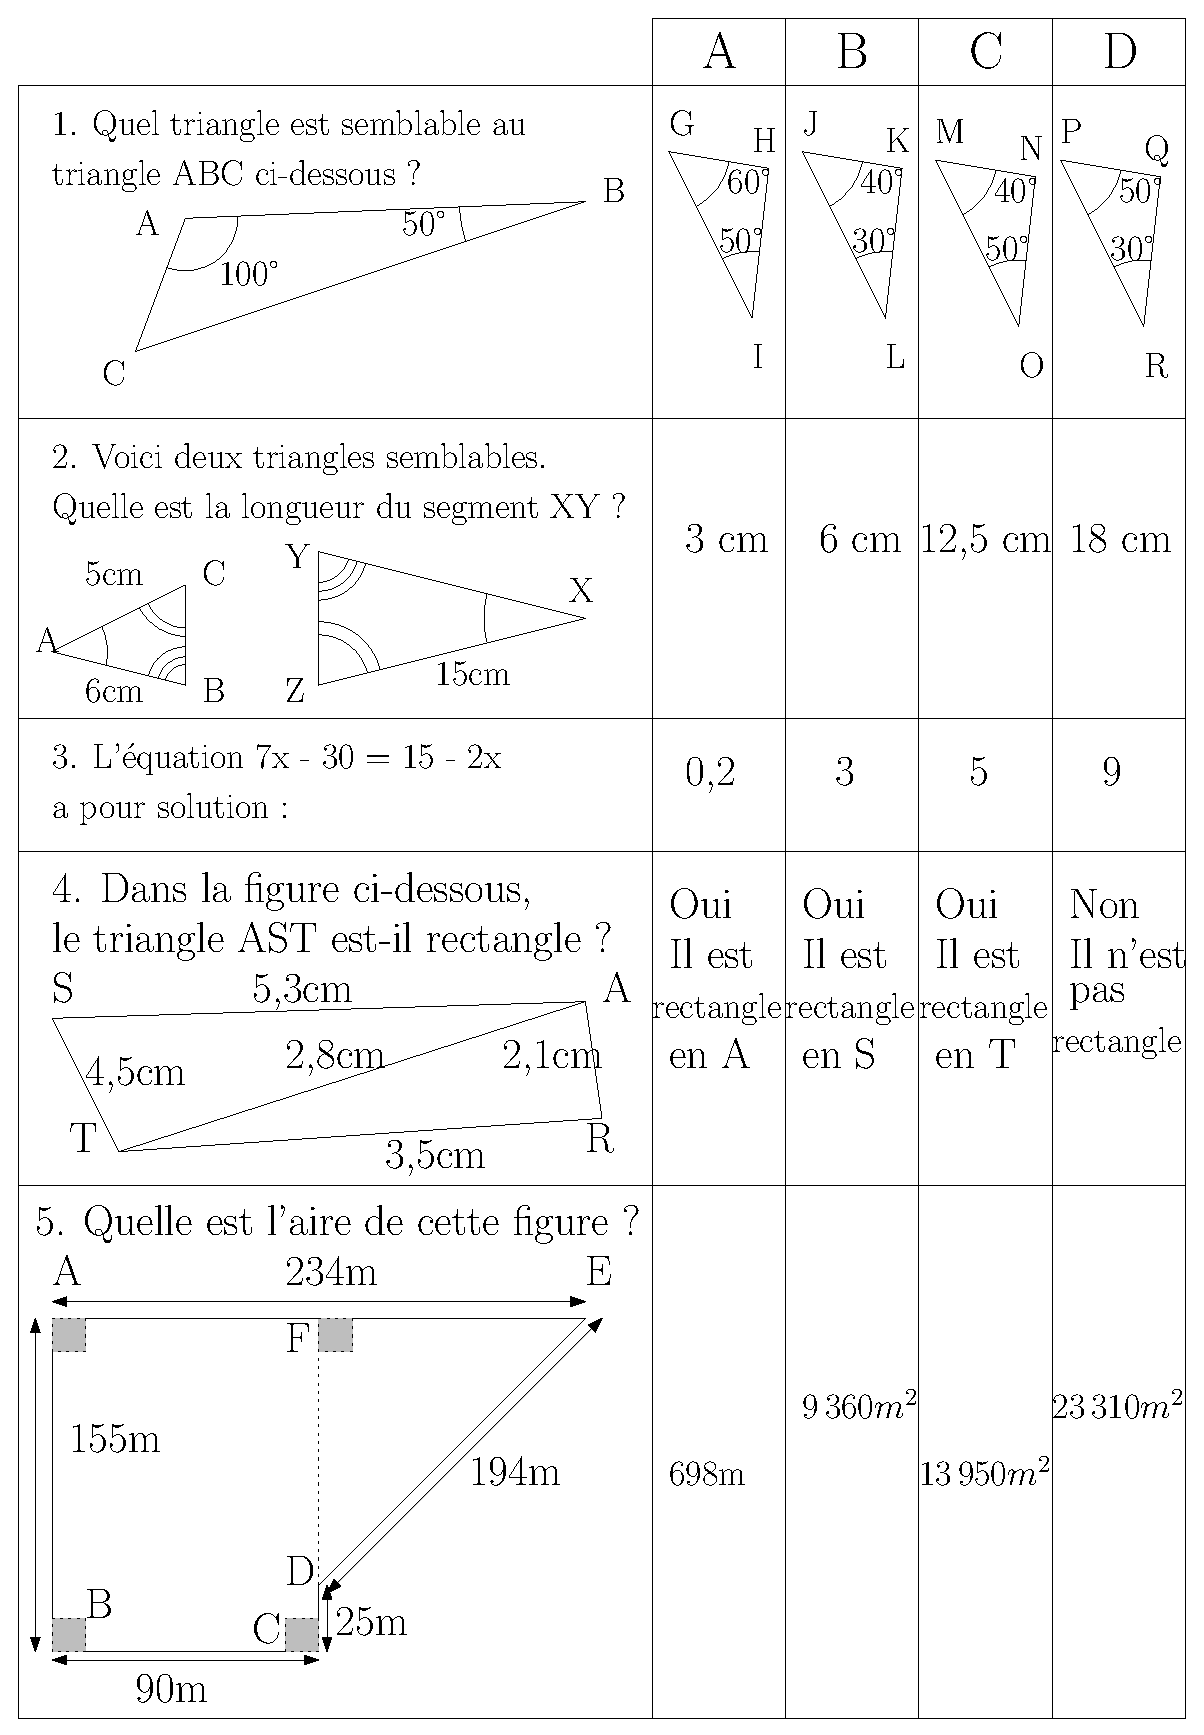
\includegraphics[width=0.8\linewidth]{qcm1-full-1.eps}
\end{figure}
\begin{figure}[H]
  \centering
  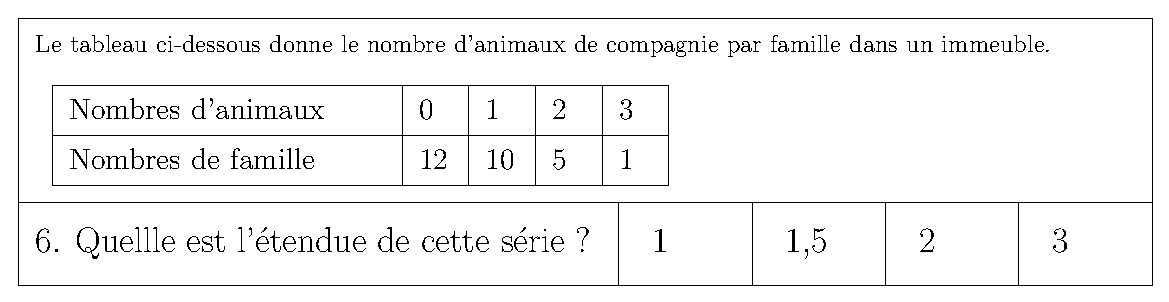
\includegraphics[width=0.8\linewidth]{qcm1-full-2.eps}
\end{figure}


\subsection*{Exercice 2 - 20 points }

\begin{tabularx}{\linewidth}{|X|l|}\hline
  Programme A &Programme B\\ \hline
  \begin{itemize}
  \item Choisir un nombre.
  \item Prendre le carré du nombre choisi.
  \item Multiplier le résultat par 2.
  \item Ajouter le double du nombre
  de départ.
  \item Soustraire 4 au résultat.
  \end{itemize}&\begin{scratch}
  \setscratch{scale=0.7,num blocks=true,print,fill blocks, fill gray=0.9}
    \blockinit{quand \greenflag est cliqué}
    \blocksensing{demander \ovalnum{Choisir un nombre}~ et attendre}
    \blockvariable{mettre \selectmenu{nombre choisi} à \ovalsensing{réponse}}
    \blockvariable{mettre \selectmenu{Résultat 1} à \ovaloperator{\ovalvariable{Nombre choisi} + \ovalnum{2} }}
    \blockvariable{mettre \selectmenu{Résultat 2} à \ovaloperator{\ovalvariable{Nombre choisi} - \ovalnum{1} }}
    \blocklook{dire \ovaloperator{regrouper \ovalnum{Le résultat est} et \ovaloperator{\ovalvariable{Résultat 1} * \ovalvariable{Résultat 2} }}}
  \end{scratch}
  \\ \hline		
  \end{tabularx}


\begin{enumerate}
  \item[1.] 
  \begin{enumerate}
    \item[a.] Vérifier que, si on choisit 5 comme nombre de départ, le résultat du programme A est 56.
    \item[b.] Quel résultat obtient-on avec le programme B si on choisit -9 comme nombre de départ ?
  \end{enumerate} 

  \item[2.] On choisit un nombre quelconque $x$ comme nombre de départ.
  \begin{enumerate}
    \item[a.] Parmi les trois propositions ci-dessous, recopier l'expression qui donne le résultat obtenu par le programme B ?
      
    \begin{multicols}{3}\noindent
      $E_1 = (x+2)-1$ \\
      $E_2 = (x+2) \times (x - 1)$ \\
      $E_3 = x + 2 \times x - 1$ 
    \end{multicols}

    \item[b.] Exprimer en fonction de $x$ le résultat obtenu avec le programme A.
  \end{enumerate} 

  \item[3.] Démontrer que, quel que soit le nombre choisi au départ, le résultat du programme A est toujours le double du résultat du programme B.
\end{enumerate}


\subsection*{Exercice 3 - 24 points }

Voici la série des temps exprimés en secondes, et réalisés par des nageuses lors de la finale du 100 mètres féminin nage libre lors des championnats d'Europe de natation de 2018 :

\begin{center}
\begin{tabularx}{\linewidth}{|*{8}{>{\centering \arraybackslash}X|}}\hline
53,23&54,04&53,61&54,52&53,35&52,93&54,56&54,07\\ \hline
\end{tabularx}
\end{center}

\begin{enumerate}
\item La nageuse française, Charlotte BONNET, est arrivée troisième à cette finale. Quel est le temps, exprimé en secondes, de cette nageuse ?
\item Quelle est la vitesse moyenne, exprimée en m/s, de la nageuse ayant parcouru les $100$ mètres en $52,93$ secondes ? Arrondir au dixième près.
\item Comparer moyenne et médiane des temps de cette série.

\newpage

Sur une feuille de calcul, on a reporté le classement des dix premiers pays selon le nombre de médailles d'or lors de ces championnats d'Europe de natation, toutes disciplines confondues :

\begin{center}
\begin{tabularx}{\linewidth}{|c|c|c|*{4}{>{\centering \arraybackslash}X|}}\hline
  &A&B &C& D &E &F\\ \hline
  1& Rang &Nation &Or 	&Argent &Bronze &Total\\ \hline
  2&1		&Russie 		&23	&15 &9 	&47 \\ \hline
  3&2		&Grande-Bretagne&13	&12 &9 	&34 \\ \hline
  4&3		&Italie 		&8	&12 &19 &39\\ \hline
  5&4		&Hongrie 		&6	&4	&2	&12\\ \hline
  6&5		&Ukraine 		&5	&6 	&2 	&13\\ \hline
  7&6		&Pays-Bas 		&5	&5 	&2 	&12\\ \hline
  8&7		&France 		&4	&2 	&6 	&12\\ \hline
  9&8		&Suède 			&4	&0 	&0 	&4\\ \hline
  10&9	&Allemagne 		&3	&6 	&10 &19\\ \hline
  11&10	&Suisse 		&1	&0 	&1 	&2\\ \hline
\end{tabularx}
\end{center}

\item Est-il vrai qu'à elles deux, la Grande-Bretagne et l'Italie ont obtenu autant de médailles d'or
que la Russie ?
\item Est-il vrai que plus de 35\,\% des médailles remportées par la France sont des médailles d'or ?
\item Quelle formule a-t-on pu saisir dans la cellule F2 de cette feuille de calcul, avant qu'elle soit
étirée vers le bas jusqu'à la cellule F11 ?

\end{enumerate}

\subsection*{Exercice 4 - 19 points }

\textbf{1\up{re} partie}

\smallskip

\parbox{0.45\linewidth}{\psset{unit=0.9cm}
\begin{pspicture}(7.4,3.6)
  %\psgrid
  \psline[linewidth=1.5pt](0,1.3)(5.3,1.3)(7,1.6)(7.4,1.8)
  \psline[linewidth=1.5pt,linestyle=dashed](6.9,1.9)(7.4,1.8)
  \psline[linewidth=1.5pt](0.6,1.7)(1.2,2)(6.5,2)(6.9,1.9)
  \psline[linewidth=1.5pt,linestyle=dashed](0,1.3)(0.6,1.7)
  \pspolygon(0,1.65)(5.3,1.65)(7.1,1.9)(7.4,2)(6.5,2.3)(1.15,2.3)
  \psline(0,0)(5.3,0)(7.1,0.2)(7.4,0.5)
  \psline[linestyle=dashed](7.4,0.5)(6.4,1.1)(1.2,1.1)(0,0)
  \psline[linestyle=dashed](6.4,1.2)(6.4,2.3)
  \psline[linestyle=dashed](1.2,1.1)(1.2,2)
  \psline(1.2,2)(1.2,2.3)
  \psline(0,1.7)(0,0)\psline(5.3,0)(5.3,1.7)\psline(7.1,0.2)(7.1,1.9)
  \psline(7.4,0.5)(7.4,2)
  \rput(6,3.3){Frise de la piscine}\psline{->}(6,3.1)(5.5,2.2)
\end{pspicture}}\hfill
\parbox{0.45\linewidth}{Une personne possède une piscine. 

Elle veut coller une frise en carrelage au niveau de la ligne d'eau.}

\medskip

La piscine vue de haut, est représentée à l'échelle par la partie grisée du schéma ci-après.

\begin{center}
\psset{unit=0.9cm}
\begin{pspicture}(10,4.5)
  \pspolygon[linewidth=1.3pt,fillstyle=solid,fillcolor=lightgray](0.5,0.5)(7.5,0.5)(9.1,1.8)(9.1,2.6)(7.5,4)(0.5,4)%HGEDBA
  \psline(7.5,0.5)(9.1,0.5)(9.1,4)(7.5,4)
  \uput[dl](0.5,0.5){H}\uput[d](7.5,0.5){G}\uput[r](9.1,1.8){E}\uput[r](9.1,2.6){D}
  \uput[u](7.5,4){B}\uput[ul](0.5,4){A}\uput[dr](9.1,0.5){F}\uput[ur](9.1,4){C}
  \rput(8.3,4){|}\rput(8.3,0.5){|}\rput{90}(9.1,3.3){|}\rput{90}(9.1,3.4){|}
  \rput{90}(9.1,1){|}\rput{90}(9.1,1.1){|}
\end{pspicture}
\end{center}


\textbf{Données :}

\smallskip

\setlength\parindent{6mm}
\begin{itemize}
\item[$\bullet~~$]le quadrilatère ACFH est un rectangle;
\item[$\bullet~~$]le point B est sur le côté [AC] et le point G est sur le côté [FH] ;
\item[$\bullet~~$]les points D et E sont sur le côté [CF] ;
\item[$\bullet~~$]AC $= 10$ m; AH $= 4$ m ; BC = FG $= 2$ m ; CD = EF $= 1,5$ m.
\end{itemize}
\setlength\parindent{0mm}

\smallskip

\textbf{Question :}

Calculer la longueur de la frise.

\newpage

\textbf{2\up{e} partie}

\smallskip
La personne décide d'installer, au-dessus de la piscine, une grande voile d'ombrage qui se compose de deux parties détachables reliées par une fermeture éclair comme le montre le schéma ci-dessous qui n'est pas à l'échelle.


\begin{multicols}{2}
  \textbf{Données :}

  \setlength\parindent{6mm}
  \begin{itemize}
    \item[$\bullet~~$]la première partie couvrant une partie de la piscine est représentée par le
    triangle KLN ;
    \item[$\bullet~~$]la deuxième partie est représentée par le trapèze LMON de bases [LN] et [MO] ;
    \item[$\bullet~~$]la fermeture éclair est représentée par le segment [LN] ;
    \item[$\bullet~~$]les poteaux : K, L et M sont alignés;
    \item[$\bullet~~$]les poteaux : K, N et O sont alignés;
    \item[$\bullet~~$]KL $= 5$ m ; LM $= 3,5$ m ; NO $= 5,25$ m ;\\ MO $= 10,2$ m et KN $= 7,5$ m.
  \end{itemize}
  \setlength\parindent{0mm}
  

\begin{center}
\psset{unit=0.7cm}
\begin{pspicture}(12,9)
  \pspolygon[fillstyle=solid,fillcolor=lightgray](-0.2,4.5)(7.2,4.5)(7.9,5.5)(7.9,6.5)(7.2,7.9)(-0.2,7.9)
  \pspolygon[fillstyle=solid,fillcolor=white](0.5,0.5)(8.4,1)(1,8.5)
  \psline[linestyle=dashed,linewidth=1.5pt](0.66,3.9)(5.5,4)
  \uput[dl](0.5,0.5){M}\uput[dr](8.4,1){O}\uput[u](1,8.5){K}
  \uput[l](0.65,3.9){L}\uput[r](5.7,4){N}
  \rput(9.5,7.5){Piscine}\psline{->}(8.8,7.4)(7.5,5.5)
  \rput(9,3){2 parties du voile d'ombrage}
  \psline{->}(6.8,3)(5.7,1.5)
  \psline{->}(6.8,3.2)(3,5)
\end{pspicture}
\end{center}

\end{multicols}



\textbf{Questions :}

\begin{enumerate}
  \item[1.] Démontrer que (LN) et (MO) sont parallèles.
  \item[2.] Calculer la longueur de la fermeture éclair.
\end{enumerate}


\subsection*{Exercice 5 - 19 points }

On veut peindre des murs d'aire inférieure à 100 m$^2$.

Voici les tarifs proposés par trois peintres en fonction de l'aire des murs à peindre en m$^2$ :

\begin{tabular}{|l l|}\hline
  \textbf{Peintre A :}& \np{150} \euro~ par m$^2$\\
  \textbf{Peintre B :}& \np{100} \euro~ par m$^2$ et \np{1000}~\euro~ d'installation de chantier\\ 
  \textbf{Peintre C :}& \np{7000} \euro~ quelle que soit l'aire inférieure à 100 m$^2$\\ \hline
\end{tabular}

\medskip

\begin{enumerate}
  \item Montrer que pour 40 m$^2$, le tarif du peintre A est de \np{6000}~\euro~, le tarif du peintre B est de \np{5000}~\euro~ et le tarif du peintre C est de \np{7000}~\euro~.
\end{enumerate}

Dans la suite de l'exercice, $x$ désigne l'aire des murs à peindre en m$^2$. 

\begin{enumerate}[resume]
  \item Écrire, en fonction de $x$, le prix proposé par le peintre B.
\end{enumerate}

Les fonctions donnant les prix proposés par le peintre B et le peintre C sont représentées sur l'\textbf{ANNEXE page 6}.

\begin{enumerate}[resume]
  \item Soient $A(x)$ et $C(x)$ les expressions des fonctions donnant le prix proposé par les peintres A et C en fonction de $x$.

On a $A(x) = \np{150}x$ et $C(x)= \np{7000}$.
	\begin{enumerate}
		\item Quelle est la nature de la fonction $A$ ?
		\item Calculer l'image de $60$ par la fonction $A$.
		\item Calculer l'antécédent de \np{3000} par la fonction $A$.
		\item Tracer la représentation graphique de la fonction $A$ sur l'\textbf{ANNEXE page 6}.
	\end{enumerate}
\item 
	\begin{enumerate}
		\item Résoudre l'équation $\np{150} x = \np{100} x + \np{1000}$. 
		\item Interpréter le résultat de la question \textbf{4. a.}
	\end{enumerate}
\item Lire graphiquement, sur l'\textbf{ANNEXE page 6}, les surfaces entre lesquelles le peintre B est le moins cher des trois peintres.
\end{enumerate}

\newpage

\textbf{Nom, Prénom : } \dotfill
\medskip \medskip

\begin{center}\textbf{ANNEXE À RENDRE AVEC LA COPIE} \end{center}
\medskip \medskip

\psset{xunit=0.145cm,yunit=0.001cm}
\begin{pspicture}(-5,-800)(90,10000)
  \psaxes[linewidth=1.25pt,Dx=5,Dy=1000]{->}(0,0)(0,0)(95,10000)

  \psline[linewidth=1.5pt](0,1000)(90,10000)
  \psline[linewidth=1.5pt](0,7000)(90,7000)


  \uput[u](84,7000){Peintre C}
  \rput{36}(80,9400){Peintre B}

  \uput[d](82,-400){surface en m$^2$}
  \uput[r](-5,10400){tarif en €}

  \multido{\n=0+5}{19}{\psline[linestyle=dotted](\n,0)(\n,10000)} 
  \multido{\n=0+1000}{11}{\psline[linestyle=dotted](0,\n)(90,\n)}

\end{pspicture}

 
\end{document}
